% Options for packages loaded elsewhere
\PassOptionsToPackage{unicode}{hyperref}
\PassOptionsToPackage{hyphens}{url}
\PassOptionsToPackage{dvipsnames,svgnames,x11names}{xcolor}
%
\documentclass[
  letterpaper,
  DIV=11,
  numbers=noendperiod]{scrartcl}

\usepackage{amsmath,amssymb}
\usepackage{iftex}
\ifPDFTeX
  \usepackage[T1]{fontenc}
  \usepackage[utf8]{inputenc}
  \usepackage{textcomp} % provide euro and other symbols
\else % if luatex or xetex
  \usepackage{unicode-math}
  \defaultfontfeatures{Scale=MatchLowercase}
  \defaultfontfeatures[\rmfamily]{Ligatures=TeX,Scale=1}
\fi
\usepackage{lmodern}
\ifPDFTeX\else  
    % xetex/luatex font selection
\fi
% Use upquote if available, for straight quotes in verbatim environments
\IfFileExists{upquote.sty}{\usepackage{upquote}}{}
\IfFileExists{microtype.sty}{% use microtype if available
  \usepackage[]{microtype}
  \UseMicrotypeSet[protrusion]{basicmath} % disable protrusion for tt fonts
}{}
\makeatletter
\@ifundefined{KOMAClassName}{% if non-KOMA class
  \IfFileExists{parskip.sty}{%
    \usepackage{parskip}
  }{% else
    \setlength{\parindent}{0pt}
    \setlength{\parskip}{6pt plus 2pt minus 1pt}}
}{% if KOMA class
  \KOMAoptions{parskip=half}}
\makeatother
\usepackage{xcolor}
\setlength{\emergencystretch}{3em} % prevent overfull lines
\setcounter{secnumdepth}{-\maxdimen} % remove section numbering
% Make \paragraph and \subparagraph free-standing
\ifx\paragraph\undefined\else
  \let\oldparagraph\paragraph
  \renewcommand{\paragraph}[1]{\oldparagraph{#1}\mbox{}}
\fi
\ifx\subparagraph\undefined\else
  \let\oldsubparagraph\subparagraph
  \renewcommand{\subparagraph}[1]{\oldsubparagraph{#1}\mbox{}}
\fi

\usepackage{color}
\usepackage{fancyvrb}
\newcommand{\VerbBar}{|}
\newcommand{\VERB}{\Verb[commandchars=\\\{\}]}
\DefineVerbatimEnvironment{Highlighting}{Verbatim}{commandchars=\\\{\}}
% Add ',fontsize=\small' for more characters per line
\usepackage{framed}
\definecolor{shadecolor}{RGB}{241,243,245}
\newenvironment{Shaded}{\begin{snugshade}}{\end{snugshade}}
\newcommand{\AlertTok}[1]{\textcolor[rgb]{0.68,0.00,0.00}{#1}}
\newcommand{\AnnotationTok}[1]{\textcolor[rgb]{0.37,0.37,0.37}{#1}}
\newcommand{\AttributeTok}[1]{\textcolor[rgb]{0.40,0.45,0.13}{#1}}
\newcommand{\BaseNTok}[1]{\textcolor[rgb]{0.68,0.00,0.00}{#1}}
\newcommand{\BuiltInTok}[1]{\textcolor[rgb]{0.00,0.23,0.31}{#1}}
\newcommand{\CharTok}[1]{\textcolor[rgb]{0.13,0.47,0.30}{#1}}
\newcommand{\CommentTok}[1]{\textcolor[rgb]{0.37,0.37,0.37}{#1}}
\newcommand{\CommentVarTok}[1]{\textcolor[rgb]{0.37,0.37,0.37}{\textit{#1}}}
\newcommand{\ConstantTok}[1]{\textcolor[rgb]{0.56,0.35,0.01}{#1}}
\newcommand{\ControlFlowTok}[1]{\textcolor[rgb]{0.00,0.23,0.31}{#1}}
\newcommand{\DataTypeTok}[1]{\textcolor[rgb]{0.68,0.00,0.00}{#1}}
\newcommand{\DecValTok}[1]{\textcolor[rgb]{0.68,0.00,0.00}{#1}}
\newcommand{\DocumentationTok}[1]{\textcolor[rgb]{0.37,0.37,0.37}{\textit{#1}}}
\newcommand{\ErrorTok}[1]{\textcolor[rgb]{0.68,0.00,0.00}{#1}}
\newcommand{\ExtensionTok}[1]{\textcolor[rgb]{0.00,0.23,0.31}{#1}}
\newcommand{\FloatTok}[1]{\textcolor[rgb]{0.68,0.00,0.00}{#1}}
\newcommand{\FunctionTok}[1]{\textcolor[rgb]{0.28,0.35,0.67}{#1}}
\newcommand{\ImportTok}[1]{\textcolor[rgb]{0.00,0.46,0.62}{#1}}
\newcommand{\InformationTok}[1]{\textcolor[rgb]{0.37,0.37,0.37}{#1}}
\newcommand{\KeywordTok}[1]{\textcolor[rgb]{0.00,0.23,0.31}{#1}}
\newcommand{\NormalTok}[1]{\textcolor[rgb]{0.00,0.23,0.31}{#1}}
\newcommand{\OperatorTok}[1]{\textcolor[rgb]{0.37,0.37,0.37}{#1}}
\newcommand{\OtherTok}[1]{\textcolor[rgb]{0.00,0.23,0.31}{#1}}
\newcommand{\PreprocessorTok}[1]{\textcolor[rgb]{0.68,0.00,0.00}{#1}}
\newcommand{\RegionMarkerTok}[1]{\textcolor[rgb]{0.00,0.23,0.31}{#1}}
\newcommand{\SpecialCharTok}[1]{\textcolor[rgb]{0.37,0.37,0.37}{#1}}
\newcommand{\SpecialStringTok}[1]{\textcolor[rgb]{0.13,0.47,0.30}{#1}}
\newcommand{\StringTok}[1]{\textcolor[rgb]{0.13,0.47,0.30}{#1}}
\newcommand{\VariableTok}[1]{\textcolor[rgb]{0.07,0.07,0.07}{#1}}
\newcommand{\VerbatimStringTok}[1]{\textcolor[rgb]{0.13,0.47,0.30}{#1}}
\newcommand{\WarningTok}[1]{\textcolor[rgb]{0.37,0.37,0.37}{\textit{#1}}}

\providecommand{\tightlist}{%
  \setlength{\itemsep}{0pt}\setlength{\parskip}{0pt}}\usepackage{longtable,booktabs,array}
\usepackage{calc} % for calculating minipage widths
% Correct order of tables after \paragraph or \subparagraph
\usepackage{etoolbox}
\makeatletter
\patchcmd\longtable{\par}{\if@noskipsec\mbox{}\fi\par}{}{}
\makeatother
% Allow footnotes in longtable head/foot
\IfFileExists{footnotehyper.sty}{\usepackage{footnotehyper}}{\usepackage{footnote}}
\makesavenoteenv{longtable}
\usepackage{graphicx}
\makeatletter
\def\maxwidth{\ifdim\Gin@nat@width>\linewidth\linewidth\else\Gin@nat@width\fi}
\def\maxheight{\ifdim\Gin@nat@height>\textheight\textheight\else\Gin@nat@height\fi}
\makeatother
% Scale images if necessary, so that they will not overflow the page
% margins by default, and it is still possible to overwrite the defaults
% using explicit options in \includegraphics[width, height, ...]{}
\setkeys{Gin}{width=\maxwidth,height=\maxheight,keepaspectratio}
% Set default figure placement to htbp
\makeatletter
\def\fps@figure{htbp}
\makeatother

\usepackage{booktabs}
\usepackage{longtable}
\usepackage{array}
\usepackage{multirow}
\usepackage{wrapfig}
\usepackage{float}
\usepackage{colortbl}
\usepackage{pdflscape}
\usepackage{tabu}
\usepackage{threeparttable}
\usepackage{threeparttablex}
\usepackage[normalem]{ulem}
\usepackage{makecell}
\usepackage{xcolor}
\KOMAoption{captions}{tableheading}
\makeatletter
\makeatother
\makeatletter
\makeatother
\makeatletter
\@ifpackageloaded{caption}{}{\usepackage{caption}}
\AtBeginDocument{%
\ifdefined\contentsname
  \renewcommand*\contentsname{Table of contents}
\else
  \newcommand\contentsname{Table of contents}
\fi
\ifdefined\listfigurename
  \renewcommand*\listfigurename{List of Figures}
\else
  \newcommand\listfigurename{List of Figures}
\fi
\ifdefined\listtablename
  \renewcommand*\listtablename{List of Tables}
\else
  \newcommand\listtablename{List of Tables}
\fi
\ifdefined\figurename
  \renewcommand*\figurename{Figure}
\else
  \newcommand\figurename{Figure}
\fi
\ifdefined\tablename
  \renewcommand*\tablename{Table}
\else
  \newcommand\tablename{Table}
\fi
}
\@ifpackageloaded{float}{}{\usepackage{float}}
\floatstyle{ruled}
\@ifundefined{c@chapter}{\newfloat{codelisting}{h}{lop}}{\newfloat{codelisting}{h}{lop}[chapter]}
\floatname{codelisting}{Listing}
\newcommand*\listoflistings{\listof{codelisting}{List of Listings}}
\makeatother
\makeatletter
\@ifpackageloaded{caption}{}{\usepackage{caption}}
\@ifpackageloaded{subcaption}{}{\usepackage{subcaption}}
\makeatother
\makeatletter
\@ifpackageloaded{tcolorbox}{}{\usepackage[skins,breakable]{tcolorbox}}
\makeatother
\makeatletter
\@ifundefined{shadecolor}{\definecolor{shadecolor}{rgb}{.97, .97, .97}}
\makeatother
\makeatletter
\makeatother
\makeatletter
\makeatother
\ifLuaTeX
  \usepackage{selnolig}  % disable illegal ligatures
\fi
\IfFileExists{bookmark.sty}{\usepackage{bookmark}}{\usepackage{hyperref}}
\IfFileExists{xurl.sty}{\usepackage{xurl}}{} % add URL line breaks if available
\urlstyle{same} % disable monospaced font for URLs
\hypersetup{
  pdftitle={Assignment 1},
  pdfauthor={YOUR NAME HERE},
  colorlinks=true,
  linkcolor={blue},
  filecolor={Maroon},
  citecolor={Blue},
  urlcolor={Blue},
  pdfcreator={LaTeX via pandoc}}

\title{Assignment 1}
\author{YOUR NAME HERE}
\date{Invalid Date}

\begin{document}
\maketitle
\ifdefined\Shaded\renewenvironment{Shaded}{\begin{tcolorbox}[frame hidden, boxrule=0pt, sharp corners, breakable, enhanced, borderline west={3pt}{0pt}{shadecolor}, interior hidden]}{\end{tcolorbox}}\fi

\hypertarget{questions}{%
\subsection{Questions}\label{questions}}

1. Using the \texttt{vtable} package, create a table of summary
statistics from the \texttt{econmath} data that includes the mean,
standard deviation, minimum, and maximum for variables: \emph{score},
\emph{hsgpa}, \emph{study}, \emph{age}.

\begin{Shaded}
\begin{Highlighting}[]
\NormalTok{econmath }\SpecialCharTok{\%\textgreater{}\%} 
  \FunctionTok{select}\NormalTok{(score, hsgpa, study, age) }\SpecialCharTok{\%\textgreater{}\%} 
  \FunctionTok{sumtable}\NormalTok{(}\AttributeTok{summ=}\FunctionTok{c}\NormalTok{(}\StringTok{\textquotesingle{}mean(x)\textquotesingle{}}\NormalTok{,}\StringTok{\textquotesingle{}sd(x)\textquotesingle{}}\NormalTok{,}\StringTok{\textquotesingle{}min(x)\textquotesingle{}}\NormalTok{,}\StringTok{\textquotesingle{}max(x)\textquotesingle{}}\NormalTok{))}
\end{Highlighting}
\end{Shaded}

\begin{table}

\caption{Summary Statistics}
\centering
\begin{tabular}[t]{lllll}
\toprule
Variable & Mean & Sd & Min & Max\\
\midrule
score & 73 & 13 & 20 & 98\\
hsgpa & 3.3 & 0.34 & 2.4 & 4.3\\
study & 14 & 7.8 & 0 & 50\\
age & 19 & 0.94 & 18 & 29\\
\bottomrule
\end{tabular}
\end{table}

2. Compute the summary statistics table as you did in (1), but group the
data by whether or not the student took a high school economics course.
Comment on the differences across groups in the mean of these variables.

INSERT COMMENTS HERE

\begin{Shaded}
\begin{Highlighting}[]
\NormalTok{econmath }\SpecialCharTok{\%\textgreater{}\%} 
  \FunctionTok{select}\NormalTok{(score, hsgpa, study, age, econhs) }\SpecialCharTok{\%\textgreater{}\%} 
  \FunctionTok{sumtable}\NormalTok{(}\AttributeTok{summ=}\FunctionTok{c}\NormalTok{(}\StringTok{\textquotesingle{}mean(x)\textquotesingle{}}\NormalTok{,}\StringTok{\textquotesingle{}sd(x)\textquotesingle{}}\NormalTok{,}\StringTok{\textquotesingle{}min(x)\textquotesingle{}}\NormalTok{,}\StringTok{\textquotesingle{}max(x)\textquotesingle{}}\NormalTok{),}
           \AttributeTok{group =} \StringTok{\textquotesingle{}econhs\textquotesingle{}}\NormalTok{)}
\end{Highlighting}
\end{Shaded}

\begin{table}

\caption{Summary Statistics}
\centering
\begin{tabular}[t]{lllllllll}
\toprule
\multicolumn{1}{c}{econhs} & \multicolumn{4}{c}{0} & \multicolumn{4}{c}{1} \\
\cmidrule(l{3pt}r{3pt}){1-1} \cmidrule(l{3pt}r{3pt}){2-5} \cmidrule(l{3pt}r{3pt}){6-9}
Variable & Mean & Sd & Min & Max & Mean & Sd & Min & Max\\
\midrule
score & 73 & 13 & 20 & 98 & 72 & 13 & 23 & 96\\
hsgpa & 3.3 & 0.34 & 2.4 & 4.1 & 3.4 & 0.35 & 2.4 & 4.3\\
study & 14 & 7.7 & 0 & 48 & 14 & 8 & 0 & 50\\
age & 19 & 0.94 & 18 & 29 & 19 & 0.94 & 18 & 28\\
\bottomrule
\end{tabular}
\end{table}

3. Using the \texttt{ggplot2} package, produce a violin plot of
\emph{score} across the two values of \emph{econhs} (note, you may need
to look up violin plots to familiarize yourself with them). Create a
title for the graph and relabel the x and y axes with more intuitive
names. Describe the relationship between these two variables. {[}NOTE:
when you define the aesthetics in your plot, you will need to declare
\emph{econhs} as a factor variable using \texttt{as.factor(econhs)}{]}

INSERT COMMENTS HERE

\begin{Shaded}
\begin{Highlighting}[]
\FunctionTok{ggplot}\NormalTok{(econmath, }\FunctionTok{aes}\NormalTok{(}\AttributeTok{y =}\NormalTok{ hsgpa, }\AttributeTok{x =} \FunctionTok{as.factor}\NormalTok{(econhs))) }\SpecialCharTok{+}
  \FunctionTok{geom\_violin}\NormalTok{() }\SpecialCharTok{+}
  \FunctionTok{labs}\NormalTok{(}\AttributeTok{title =} \StringTok{"Density of Economics Scores"}\NormalTok{, }
       \AttributeTok{x =} \StringTok{"High School GPA"}\NormalTok{, }\AttributeTok{y =} \StringTok{"Density"}\NormalTok{)}
\end{Highlighting}
\end{Shaded}

\begin{figure}[H]

{\centering 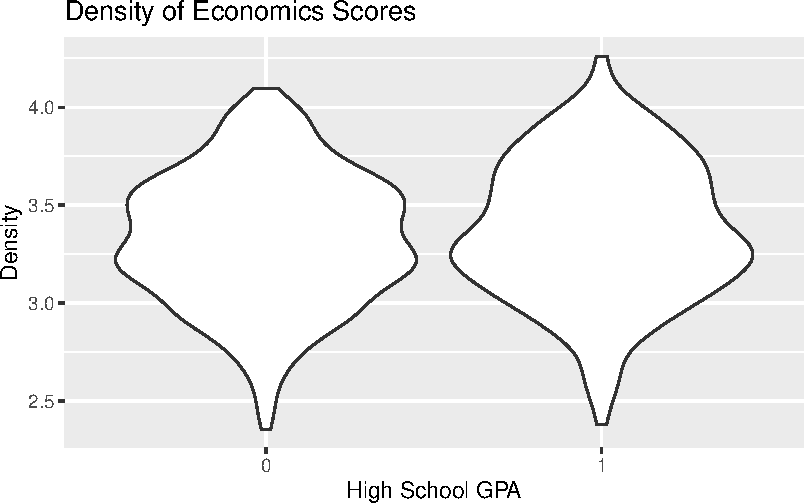
\includegraphics{a1template_files/figure-pdf/unnamed-chunk-4-1.pdf}

}

\end{figure}

4. Using the \texttt{ggplot2} package, produce a scatterplot with
\emph{score} on the y-axis and \emph{hsgpa} on the x-axis. Layer on top
of that a \textbf{loess} regression line (again, look up what a loess
function is). Create a title for the graph and relabel the x and y axes
with more intuitive names. Describe the relationship between these two
variables.

INSERT COMMENTS HERE

\begin{Shaded}
\begin{Highlighting}[]
\NormalTok{p}\OtherTok{\textless{}{-}}\FunctionTok{ggplot}\NormalTok{(econmath, }\FunctionTok{aes}\NormalTok{(}\AttributeTok{y =}\NormalTok{ score, }\AttributeTok{x =}\NormalTok{ hsgpa)) }\SpecialCharTok{+}
  \FunctionTok{geom\_point}\NormalTok{() }\SpecialCharTok{+}
  \FunctionTok{geom\_smooth}\NormalTok{(}\AttributeTok{method =} \StringTok{"loess"}\NormalTok{) }\SpecialCharTok{+}
  \FunctionTok{labs}\NormalTok{(}\AttributeTok{title =} \StringTok{"Economics Grades and High School GPA"}\NormalTok{, }
       \AttributeTok{x =} \StringTok{"High School GPA"}\NormalTok{, }\AttributeTok{y =} \StringTok{"Economics Score"}\NormalTok{)}
\NormalTok{p}
\end{Highlighting}
\end{Shaded}

\begin{verbatim}
`geom_smooth()` using formula = 'y ~ x'
\end{verbatim}

\begin{figure}[H]

{\centering 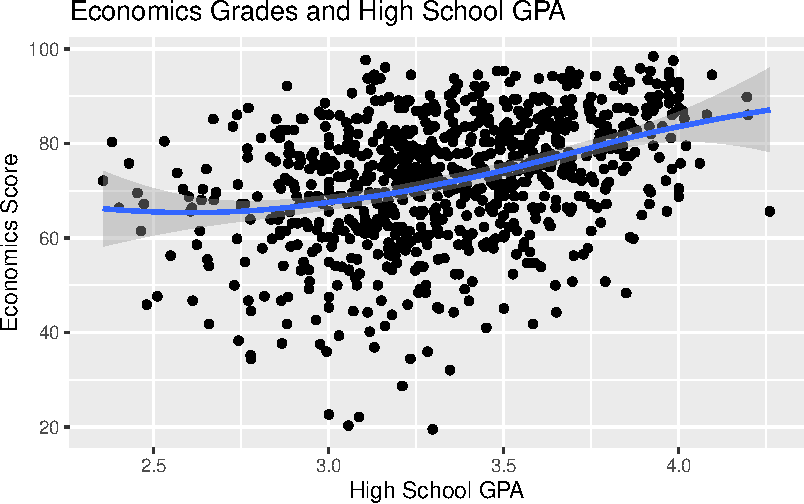
\includegraphics{a1template_files/figure-pdf/unnamed-chunk-5-1.pdf}

}

\end{figure}

5. Suppose that the process that generates a set of data is
\(y = 1 + x + 0.5*x^2 + \epsilon\), where
\(\epsilon \sim \mathcal{N}(0,40^2)\), and
\(x \sim \mathcal{N}(30,5^2)\). This means that the Conditional
Expectation Function (CEF) is \(E[y|x] = 1 + x + 0.5*x^2\). The code
below creates the data for \(x\) and \(y\). Plot the conditional
expectation function on top of a scatterplot of the data.

\begin{Shaded}
\begin{Highlighting}[]
\NormalTok{data }\OtherTok{\textless{}{-}} \FunctionTok{tibble}\NormalTok{(}\AttributeTok{x =} \FunctionTok{rnorm}\NormalTok{(}\DecValTok{1000}\NormalTok{,}\DecValTok{30}\NormalTok{,}\DecValTok{5}\NormalTok{),}
               \AttributeTok{y =} \DecValTok{1} \SpecialCharTok{+}\NormalTok{ x }\SpecialCharTok{+} \FloatTok{0.5}\SpecialCharTok{*}\NormalTok{x}\SpecialCharTok{\^{}}\DecValTok{2} \SpecialCharTok{+} \FunctionTok{rnorm}\NormalTok{(}\DecValTok{1000}\NormalTok{,}\DecValTok{0}\NormalTok{,}\DecValTok{40}\NormalTok{))}

\FunctionTok{ggplot}\NormalTok{(data, }\FunctionTok{aes}\NormalTok{(}\AttributeTok{x =}\NormalTok{ x, }\AttributeTok{y =}\NormalTok{ y)) }\SpecialCharTok{+} 
  \FunctionTok{geom\_point}\NormalTok{() }\SpecialCharTok{+} 
  \FunctionTok{geom\_function}\NormalTok{(}\AttributeTok{fun =} \ControlFlowTok{function}\NormalTok{(x) }\DecValTok{1} \SpecialCharTok{+}\NormalTok{ x }\SpecialCharTok{+} \FloatTok{0.5}\SpecialCharTok{*}\NormalTok{x}\SpecialCharTok{\^{}}\DecValTok{2}\NormalTok{)}
\end{Highlighting}
\end{Shaded}

\begin{figure}[H]

{\centering 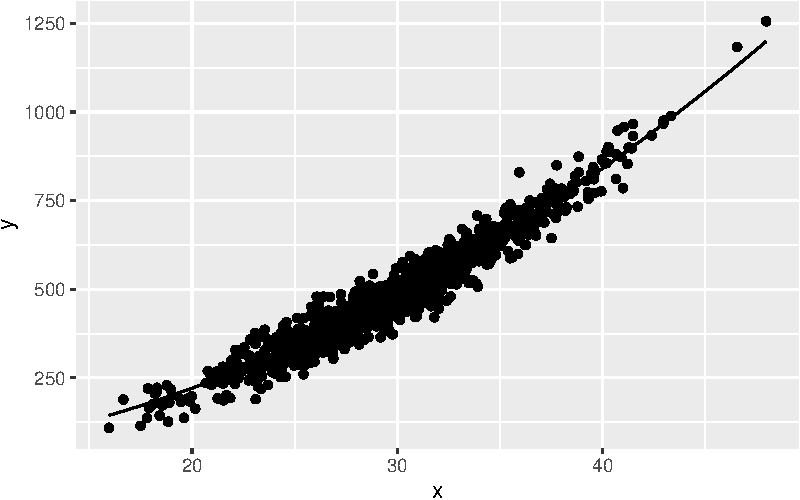
\includegraphics{a1template_files/figure-pdf/unnamed-chunk-6-1.pdf}

}

\end{figure}

6. Suppose you are interested in the Population Regression of \(y\) on
\(x\) as an approximation of the CEF. Compute the population regression
slope and intercept. A useful piece of information for this question is
that for a Normal random variable \(x\), the covariance between \(x\)
and \(x^2\) is \((E[x])^3 + 3E[x]Var[x] - E[x]((E[x])^2+ Var[x])\).

INSERT COMMENTS HERE

7. Plot the Population Regression Function (PRF) with the CEF and
comment on the quality of the approximation.

INSERT COMMENTS HERE

\begin{Shaded}
\begin{Highlighting}[]
\FunctionTok{ggplot}\NormalTok{() }\SpecialCharTok{+} 
  \FunctionTok{geom\_function}\NormalTok{(}\AttributeTok{fun =} \ControlFlowTok{function}\NormalTok{(x) }\DecValTok{1} \SpecialCharTok{+}\NormalTok{ x }\SpecialCharTok{+} \FloatTok{0.5}\SpecialCharTok{*}\NormalTok{x}\SpecialCharTok{\^{}}\DecValTok{2}\NormalTok{) }\SpecialCharTok{+}
  \FunctionTok{geom\_function}\NormalTok{(}\AttributeTok{fun =} \ControlFlowTok{function}\NormalTok{(x) }\SpecialCharTok{{-}}\FloatTok{436.5} \SpecialCharTok{+} \DecValTok{31}\SpecialCharTok{*}\NormalTok{x ) }\SpecialCharTok{+} 
  \FunctionTok{xlim}\NormalTok{(}\DecValTok{0}\NormalTok{,}\DecValTok{50}\NormalTok{)}
\end{Highlighting}
\end{Shaded}

\begin{figure}[H]

{\centering 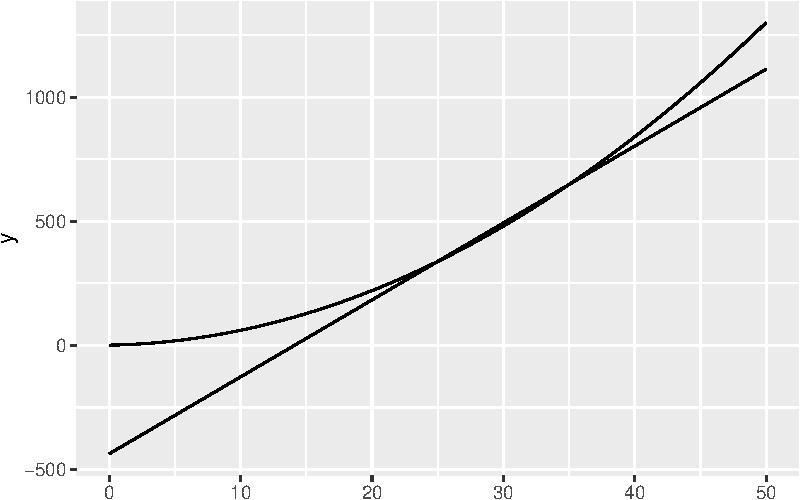
\includegraphics{a1template_files/figure-pdf/unnamed-chunk-7-1.pdf}

}

\end{figure}



\end{document}
